\documentclass{article}
\usepackage[margin=1.25in]{geometry}
\usepackage{amsmath, amssymb, setspace, enumerate, enumitem}
\usepackage{setspace}
\usepackage{graphicx}
\onehalfspacing

\begin{document}
    \begin{enumerate}
        \item Exercise 3.4
        \begin{enumerate}[label=(\alph*)]
            \item we know $y = w^{*T}X + \epsilon$ and $H = X(X^TX)^-1X^T$ from (3.6), and we know $\hat{y} = Hy$ by definition, we want to prove $\hat{y} = Xw^* + H\epsilon$
            \begin{align*}
                \hat{y} &= H(w^*X + \epsilon)\\
                &= X(X^TX)^{-1}X^T(w^*X+\epsilon)\\
                &= X(X^TX)^{-1}X^Tw^*X + X(X^TX)^{-1}X^T\epsilon\\
                &= w^*X + H\epsilon
            \end{align*}

            \item for $\hat{y} - y$, we have
            \begin{align*}
                \hat{y} - y &= w^*X + H\epsilon - (w^*X + \epsilon)\\
                &= H\epsilon - \epsilon\\
                &= \epsilon(H - I)
            \end{align*}
            where $I$ denotes the identity matrix
            
            \item let $E_{in}(w) = \frac{1}{N} ||\hat{y} - y||^2$
            \begin{align*}
                E_{in}(w) &= \frac{1}{N}||\epsilon(H-I)||^2\\
                &= \frac{1}{N}(\epsilon(H - I))^T(\epsilon(H - I))\\
                &= \frac{1}{N}\epsilon^T(H-I)^T\epsilon(H-I)\\
            \end{align*}
            We know $H - I$ is symmetric, so $(H-I)^T = (H-I)$
            \begin{align*}
                E_{in}(w) &= \frac{1}{N}\epsilon^T\epsilon(H-I)^2\\
                &= \frac{1}{N}\epsilon^T\epsilon(I - H)^2
            \end{align*}

            \item We know
            \begin{align*}
                E_D[E_{in}(w_{lin})] &= E_D[\frac{1}{N}(\epsilon^T\epsilon(I - H))]\\
                &= \frac{1}{N} (E_D[\epsilon^T\epsilon] - E_D[\epsilon^T\epsilon H])\\
            \end{align*}
            Given that $\epsilon$ is a noise term with zero mean and $\sigma^2$ variance. The variance of each noise component $\epsilon$ is $\sigma^2$, so 
            \begin{align*}
                E_D[E_{in}(w_{lin})] &= \frac{1}{N}(N\sigma^2 - E_D[\epsilon^T\epsilon H])\\
                &= \sigma^2 - \frac{1}{N}E_D[\epsilon^T\epsilon H]
            \end{align*}
            
            Now we can calculate
            \begin{align*}
                E_D[\epsilon^T\epsilon H] &= E_D[\sum_{i = 1}^{N}\epsilon_i^2 H]\\
                &= H \sum_{i = 1}^{N}E_D[\epsilon_i^2]
            \end{align*}

            By the problem, we know that each component of $\epsilon$ is a random variable with zero mean and variance $\sigma^2$, so this means that $E_D[\epsilon_i] = 0$ and $E_D[\epsilon_i^2] = \sigma^2$ for all $i$.
            \begin{align*}
                E_D[\epsilon^T\epsilon H] &= H\sum_{i = 1}^{N} \sigma^2\\
                &= HN\sigma^2
            \end{align*}

            We continue the problem by substituting the result into our original equation
            \begin{align*}
                E_D[E_{in}(w_{lin})] = \sigma^2 - \frac{1}{N} E_D[\epsilon^T\epsilon H] &= \sigma^2 - \frac{1}{N}HN\sigma^2\\
                &= \sigma^2 - H\sigma^2
            \end{align*}

            Then, we can calculate for the $trace(H)$
            \begin{align*}
                trace(H) &= trace(X(X^T X)^{-1} X^T)\\
                &= trace((X^TX)^{-1}(X^TX))
            \end{align*}

            Given that $X^T X$ is a square matrix of size $(d + 1)$, and it's inverse $(X^TX)^{-1}$ is also present, then we have
            \begin{align*}
                trace((X^TX)^{-1}(X^TX)) &= d + 1\\
                trace(H) &= \frac{d + 1}{N}
            \end{align*}

            Then, we have proved that $E_D[E_{in}(w_{lin})] = \sigma^2 ( 1 - \frac{d + 1}{N}) \hfill\blacksquare$
            
            \item to do...
            
        \end{enumerate}

        \item Problem 3.1
        \begin{enumerate}[label=(\alph*)]
            \item 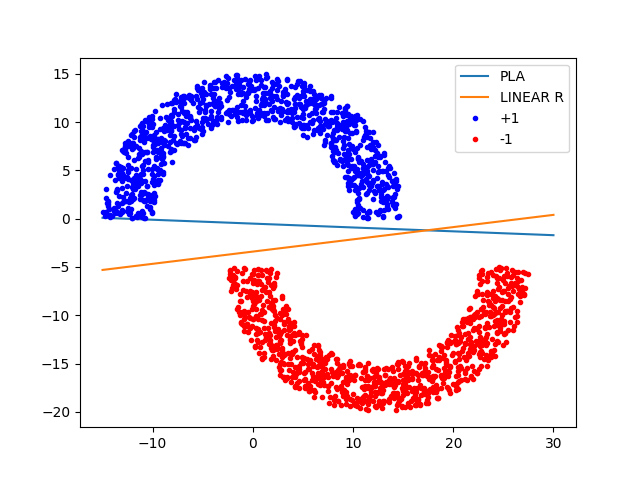
\includegraphics[scale=0.5]{images/p3_1.png}
            \item Both PLA and linear regression found ways to separate this data, however, one could say that the linear regression algorithm found a better way to separate the data as the PLA appears to be closer to the top part of the semicircle, barely missing on misclassifying one of the $+1$ points. With this, one can predict that linear regression will have a lower $E_{out}$ than the PLA, however, this isn't guaranteed.
        \end{enumerate}

        \item Problem 3.2\\
        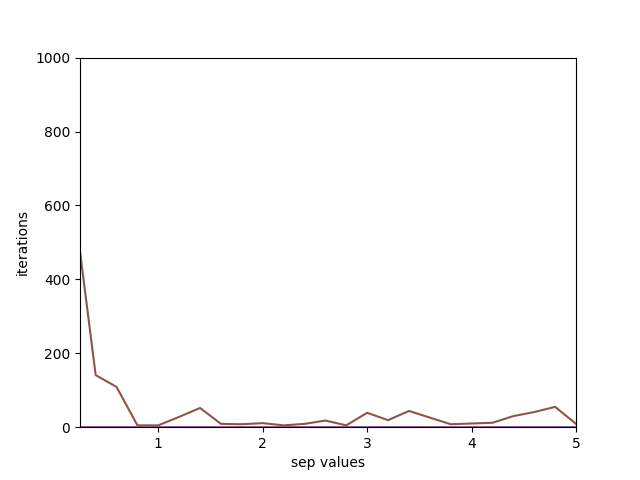
\includegraphics[scale=0.5]{images/p3_2.png}\\
        When $sep$ is small, we require a large number of iterations to find the line of best fit. When the separation between the data sets is larger, iterations decrease significantly. Intuitively, we can give this reasoning due to the number of possible hypothesis when you have a larger gap between the two datasets. When $sep$ is high, we can imagine a large gap between the two datasets, and any line inside of that gap can fit. However, when $sep$ is small, we need the perfect line to fit in between the dataset, which limits how many lines are possible, thus causing PLA to run more iterations.\\[0.25in]
        Mathematically, we proved that
        \begin{align*}
            t \leq \frac{R^2 ||w^*||^2}{p^2}
        \end{align*}
        Our sep values increase with our $p$, so as $sep$ grows larger, $p$ grows larger, creating a smaller bound for our iterations $t$.

        \item Problem 3.8\\
        Out of sample error $E_{out}(h) = E[(h(x) - y)^2]$, the hypothesis that minimizes $E_{out}$ is given by $h^*(x) = E[y|x]$. We can write $y = h^*(x) + \epsilon (x)$, where $\epsilon (x)$ is a noise variable. To minimize $E_{out}$, we can take its derivative and set it to 0
        \begin{align*}
            E[(h(x) - y)^2] &= E[h(x)^2 - 2h(x)y + y^2]\\
            \frac{d}{dh(x)}E[(h(x) - y)^2] &= 2E[(h(x) - y)]\\
            &= E[h(x) - y]\\
            &= h(x) - E[y|x]\\
            h(x) - E[y|x] &= 0\\
            h(x) &= E[y|x]
        \end{align*}

        To show that $\epsilon (x)$ has expected value zero, we do the following:
        \begin{align*}
            y &= h^*(x) + \epsilon (x)\\
            E[y] &= E[h^*(x) + \epsilon (x)]\\
            &= E[h^*(x)] + E[\epsilon (x)]\\
            E[\epsilon(x)] &= E[y] - E[h^*(x)]\\
        \end{align*}
        We know that $E[y]$ is the target function and $E[h^*(x)]$ is the closest approximate to $E[y]$ since it minimizes $E_{out}$, therefore, we can assume $E[\epsilon (x)] = 0$ since the difference between $E[y]$ and $E[h^*(x)]$ should be minimal.

        \item Handwriting
        \begin{enumerate}[label=(\alph*)]
            \item 
\includegraphics[scale=0.5]{images/3_8_1.png}\\ 
\includegraphics[scale=0.5]{images/3_8_5.png}
            \item I will be using symmetry and average intensity for my features, for symmetry, I will measure horizontal and vertical symmetry, and then get their difference, since $1$ has high symmetry on both vertical and horizontal, it should obtain a rather small difference compared to $5$\\[0.25in]
            Mathematically, assume pixels are from 0-15, rows 0-15, then horizontal symmetry can be measured by comparing the first pixel i = 0, j = 0 to pixel i = 15, j = 0, and so on until the row is completed, then the top half will drop a row while the bottom half will rise a row. This will terminate until they reach the middle. The same will happen for vertical.
            \begin{align}
                \sum_{i = 0}^{7} \sum_{j = 0}^{15} &= | p[i][j] - p[15 - i][j] |\\
                \sum_{i = 0}^{15} \sum_{j = 0}^{7} &= | p[i][j] - p[i][15 - j] |
            \end{align}

            $(1)$ horizontal
            $(2)$ vertical

            \item training plot: \\ 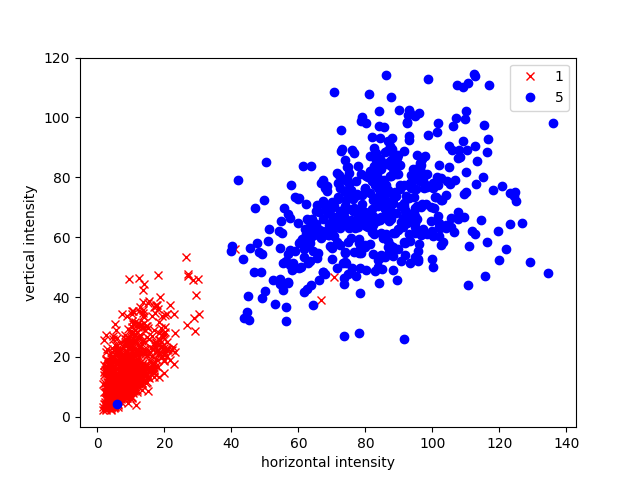
\includegraphics[scale=0.5]{images/handwriting_train.png}\\
            testing plot: \\ 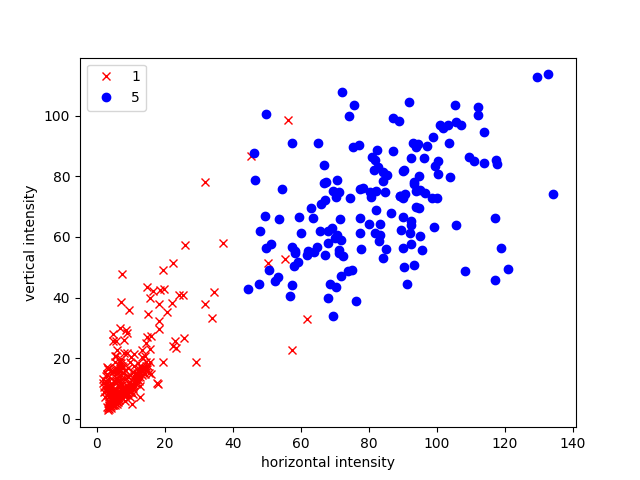
\includegraphics[scale=0.5]{images/handwriting_test.png}
        \end{enumerate}
    \end{enumerate}
\end{document}